\documentclass[11pt, oneside]{article}   	% use "amsart" instead of "article" for AMSLaTeX format
\usepackage{geometry}                		% See geometry.pdf to learn the layout options. There are lots.
\geometry{letterpaper}                   		% ... or a4paper or a5paper or ... 
%\geometry{landscape}                		% Activate for for rotated page geometry
%\usepackage[parfill]{parskip}    		% Activate to begin paragraphs with an empty line rather than an indent
\usepackage{graphicx}				% Use pdf, png, jpg, or eps� with pdflatex; use eps in DVI mode
								% TeX will automatically convert eps --> pdf in pdflatex		
\usepackage{amssymb}
\usepackage{amsmath}
\usepackage{parskip}
\usepackage{color}

\title{Differentiability and Continuity}
%\author{The Author}
%\section{}
% \subsection*{R code}
\date{}							% Activate to display a given date or no date

\graphicspath{{/Users/telliott_admin/Dropbox/Tex/png/}}

% \begin{center} 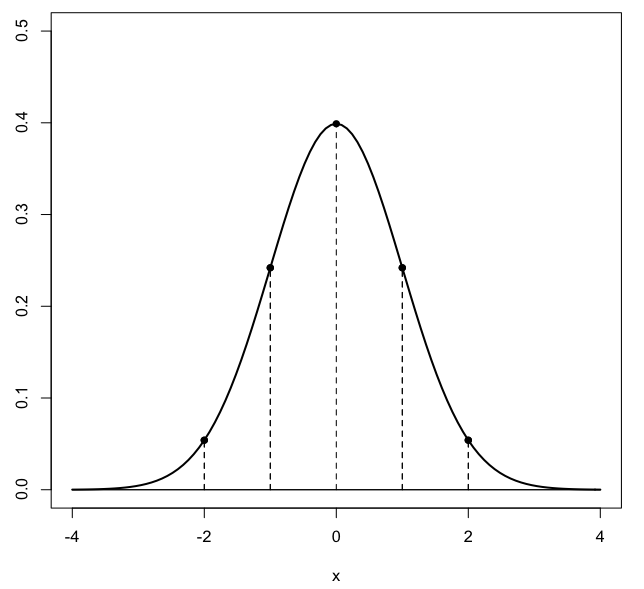
\includegraphics [scale=0.4] {gauss3.png} \end{center}
% \begin{bmatrix} a  &  b \\ c  &  d \end{bmatrix}
% \bigg |_

\begin{document}
\maketitle
\Large
%\noindent

A function is differentiable at a point $x=a$ if the derivative is defined at that point, that is if this limit

\[ f'(x) = \lim_{h \to 0} \frac{f(x+h) - f(x)}{h} \]
is defined at $x=a$, that is, if

\[ \lim_{h \to 0} \frac{f(a+h) - f(a)}{h} \]
exists.  So for example

\[ f(x) = \ln x \]
\[ f'(x) = \frac{1}{x} \]
In the above example, $f(x)$ is differentiable everywhere, except at $x=0$.

\subsection*{Continuity}

Continuity has an intuitive definition:  we should be able to graph the function \emph{without lifting the pencil from the paper}.  Basically, we require that for a function to be continuous at a point $x=a$, if we move $x$ away from $a$ by a little bit, then $f(x)$ should not change from $f(a)$ by too much.  

A formal definition uses the apparatus of limits:  epsilons and deltas.  We implement this backwards (as usual) by specifying how little the change in $f(x)$ can be, call it ($\epsilon$).  Then if we can find $\delta$, a change in $x$, such that 

\[ | f(x \pm \delta) - f(x) | < \epsilon \]
for \emph{any} $\epsilon$, we are good.

A particularly easy way to answer the question "is my function continuous at $x=a$" is to ask whether it is differentiable at $x=a$.  The reason is the following theorem:

\textcolor{blue}{If a function is differentiable at $x$, then it is continuous at $x$.}

I'm going to prove this theorem.  A semi-official statement of continuity (with no delta or epsilon) is that if

\[ \lim_{h \to 0}f(x + h) = f(x) \]
then $f$ is continuous at $x$.  And that seems perfectly clear.
So how do we get there?  For starters, notice what we're given as known, namely, that the limit

\[ f'(x) = \lim_{h \to 0} \frac{f(x+h) - f(x)}{h} \]
exists.  That's what the first part of the theorem states as \emph{given}.  And since $f'(x)$ exists, we know that $f(x)$ exists, otherwise this limit would be nonsense.

OK.  Now for the proof.  Consider

\[ \lim_{h \to 0} \frac{f(x+h) - f(x)}{h}  \times h \]
We know that this limit exists.  Why?  Because we can use the product rule for limits to split it into two parts
\[ \lim_{h \to 0} \frac{f(x+h) - f(x)}{h} \times \lim_{h \to 0} h \]
The product of these two factors is 
\[ f'(x) \times \lim_{h \to 0} h = f'(x) \times 0 = 0 \]
So the limit exists, and its value is $0$.

On the other hand, we can cancel the $h$ from the first expression, obtaining
\[ \lim_{h \to 0} f(x+h) - f(x) \]
and since we showed that the first limit exists (and is equal to zero), this second one must exist as well (and still be equal to zero).  Let's see what more we can do with this.  We can split the limit into two parts:
\[ \lim_{h \to 0} f(x+h) - \lim_{h \to 0} f(x) \]
but $h$ is not involved in the second term so
\[ \lim_{h \to 0} f(x+h) - f(x) \]
Now, we know that this whole thing is equal to $0$
\[ \lim_{h \to 0} f(x+h) - f(x) = 0 \]
Put $f(x)$ on the right-hand side, and we're done.

Remember though, that continuity does \emph{not} imply differentiability.  A counterexample is the absolute value function at $x=0$.  The function is continuous, but the slope at $x=0$ does not exist (because the slopes coming in from the two directions are not the same).



\end{document}  